\documentclass[10pt]{beamer}\usepackage[]{graphicx}\usepackage[]{color}
%% maxwidth is the original width if it is less than linewidth
%% otherwise use linewidth (to make sure the graphics do not exceed the margin)
\makeatletter
\def\maxwidth{ %
  \ifdim\Gin@nat@width>\linewidth
    \linewidth
  \else
    \Gin@nat@width
  \fi
}
\makeatother

\definecolor{fgcolor}{rgb}{0.345, 0.345, 0.345}
\newcommand{\hlnum}[1]{\textcolor[rgb]{0.686,0.059,0.569}{#1}}%
\newcommand{\hlstr}[1]{\textcolor[rgb]{0.192,0.494,0.8}{#1}}%
\newcommand{\hlcom}[1]{\textcolor[rgb]{0.678,0.584,0.686}{\textit{#1}}}%
\newcommand{\hlopt}[1]{\textcolor[rgb]{0,0,0}{#1}}%
\newcommand{\hlstd}[1]{\textcolor[rgb]{0.345,0.345,0.345}{#1}}%
\newcommand{\hlkwa}[1]{\textcolor[rgb]{0.161,0.373,0.58}{\textbf{#1}}}%
\newcommand{\hlkwb}[1]{\textcolor[rgb]{0.69,0.353,0.396}{#1}}%
\newcommand{\hlkwc}[1]{\textcolor[rgb]{0.333,0.667,0.333}{#1}}%
\newcommand{\hlkwd}[1]{\textcolor[rgb]{0.737,0.353,0.396}{\textbf{#1}}}%
\let\hlipl\hlkwb

\usepackage{framed}
\makeatletter
\newenvironment{kframe}{%
 \def\at@end@of@kframe{}%
 \ifinner\ifhmode%
  \def\at@end@of@kframe{\end{minipage}}%
  \begin{minipage}{\columnwidth}%
 \fi\fi%
 \def\FrameCommand##1{\hskip\@totalleftmargin \hskip-\fboxsep
 \colorbox{shadecolor}{##1}\hskip-\fboxsep
     % There is no \\@totalrightmargin, so:
     \hskip-\linewidth \hskip-\@totalleftmargin \hskip\columnwidth}%
 \MakeFramed {\advance\hsize-\width
   \@totalleftmargin\z@ \linewidth\hsize
   \@setminipage}}%
 {\par\unskip\endMakeFramed%
 \at@end@of@kframe}
\makeatother

\definecolor{shadecolor}{rgb}{.97, .97, .97}
\definecolor{messagecolor}{rgb}{0, 0, 0}
\definecolor{warningcolor}{rgb}{1, 0, 1}
\definecolor{errorcolor}{rgb}{1, 0, 0}
\newenvironment{knitrout}{}{} % an empty environment to be redefined in TeX

\usepackage{alltt}%
\usetheme{Boadilla}
\usecolortheme{seahorse}

\usepackage[utf8]{inputenc}%

% graphics
%% Figures %%%%%%%%%%%%%%%%%%%%%%%%%%%%%%%%%%%%%%%%%%%%%%%%%%
\usepackage{graphicx}
\usepackage{xcolor}%for color mixing

\usepackage{amsmath}%
\usepackage{amsfonts}%
\usepackage{amssymb}%
\usepackage{graphicx}

\usepackage{tikz}

%%%%%%%%%%%%%%%%%%%%%%%%%%%%%%%%%%%%%%%%%%%%%%
%%%%%%%%%%%%%%%%% Doc info %%%%%%%%%%%%%%%%%%%
\title[\textbf{Linear models}]{Statistical inference and linear models}
\date{\today}

%%%%%%%%%%%%%%%%%%%%%%%%%%%%%%%%%%%%
\IfFileExists{upquote.sty}{\usepackage{upquote}}{}
\begin{document}




\begin{frame}
\maketitle	
\end{frame}
%%%%%%%%%%%

\AtBeginSection[]
{
  \begin{frame}<beamer>
    \frametitle{}
    \tableofcontents[currentsection,hideothersubsections,subsectionstyle=hide]% down vote\tableofcontents[currentsection,currentsubsection,hideothersubsections,sectionstyle=show/hide,subsectionstyle=show/shaded/hide] 
  \end{frame}
} 

\begin{frame}{If you get bored}
  \begin{itemize}
    \item Go to the last slide for bonus exercises
    \item Work on code for your research and ask question during exercise time
    \item But try and keep an eye out, just in case
  \end{itemize}
  
  \begin{center}
    
\includegraphics[height=0.5\textheight]{Figures/too-easy-whats-next.jpg}
  \end{center}
\end{frame}
%%%%%%%%%%%

\begin{frame}{Disclaimer}
  \begin{itemize}
    \item Assume you got lectures about statistics and
       \begin{itemize}
        \item know why we need statistics
        \item have heard of the general philosophy
       \end{itemize}
    \item We may simplify to focus on practical aspects
    \item Correct us if we say something completely awful
  \end{itemize}
  
\end{frame}
%%%%%%%%%%%

\section{Statistical inference}%very general, still simplistic

\begin{frame}{General approach}

\begin{center}
  \begin{tikzpicture}
    \node (sq) at (0,-1) {\color{red}{1. Scientific question}};
    \pause
    \node (mo) at (0,-2) {2. Model and Statistical question};
    \draw[->, thick] (sq)--(mo);
    \pause
    \node (dac) at (6,-2) {\color{red}{3. Data collection}};
    \draw[<->, thick] (mo)--(dac);
    \pause
    \node (est) at (0,-3) {4. Estimation};
        \draw[->, thick] (mo)--(est);
    \node (unc) at (0,-3.5) {4.b Uncertainty and statistical significance};
    \pause
    
    \node (che) at (0,-5) {5. Diagnostic, check assumptions, prediction};
        \draw[->, thick] (unc)--(che);
    \draw[->, thick] (che.west) to [out=150, in=210] (mo.west);

    \pause
    \node (int) at (0,-6) {\color{red}{6. Interpret and think about the biology}};
        \draw[->, thick] (che)--(int);

  \draw[rounded corners, color=blue] (-4.5,-1.5) rectangle (4,-5.5);
  \node[anchor=north west] (r) at (-4.5,-1.5) {
\includegraphics[width=0.1\textwidth]{Figures/r}};
  \end{tikzpicture}
  \end{center}
\end{frame}
%%%%%%%%%%%

\begin{frame}[fragile]{Reminder t.test}
  
  \pause
\begin{knitrout}
\definecolor{shadecolor}{rgb}{0.843, 0.867, 0.922}\color{fgcolor}\begin{kframe}
\begin{alltt}
  \hlkwd{data}\hlstd{(}\hlstr{"iris"}\hlstd{)}
\end{alltt}
\end{kframe}
\end{knitrout}

\begin{knitrout}
\definecolor{shadecolor}{rgb}{0.843, 0.867, 0.922}\color{fgcolor}\begin{kframe}
\begin{alltt}
  \hlkwd{str}\hlstd{(iris)}
  \hlkwd{plot}\hlstd{(iris)}
\end{alltt}
\end{kframe}
\end{knitrout}
  
  \begin{enumerate}
    \item \color{red}{Scientific question}: Are the taxa "setosa" and "versicolor" different species?
  \pause
    \item Model and stat question:
      \begin{itemize}
        \item Model:
          \begin{itemize}
            \item There is an intrinsic/expected sepal length value for a species; an individual value is the sum of this expectation and a random Gaussian deviation.
            \item $y_i = \mu_{species_i} + \epsilon_i$ with  $\epsilon \sim N(0,\sigma^2)$
            \item t-test
          \end{itemize}
        \pause
        \item Statistical question: 
          \begin{itemize}
            \item Does sepal length \textbf{differ significantly} between the two taxa \textbf{in our sample}?
            \item Is the observed difference between taxa likely if both taxa have the same intrinsic/expected value?
          \end{itemize}
        \end{itemize}
      \item Data collection
    \end{enumerate}
\end{frame}
%%%%%%%%%%%

\begin{frame}[fragile]{Reminder t.test}
    One t-test for sepal length between \textit{setosa} and \textit{versicolor}:
\begin{knitrout}
\definecolor{shadecolor}{rgb}{0.843, 0.867, 0.922}\color{fgcolor}\begin{kframe}
\begin{alltt}
  \hlkwd{t.test}\hlstd{(}\hlkwc{x} \hlstd{= iris}\hlopt{$}\hlstd{Sepal.Length[iris}\hlopt{$}\hlstd{Species} \hlopt{==} \hlstr{"setosa"}\hlstd{],}
        \hlkwc{y} \hlstd{= iris}\hlopt{$}\hlstd{Sepal.Length[iris}\hlopt{$}\hlstd{Species} \hlopt{==} \hlstr{"versicolor"}\hlstd{])}
\end{alltt}
\begin{verbatim}

	Welch Two Sample t-test

data:  iris$Sepal.Length[iris$Species == "setosa"] and iris$Sepal.Length[iris$Species == "versicolor"]
t = -10.521, df = 86.538, p-value < 2.2e-16
alternative hypothesis: true difference in means is not equal to 0
95 percent confidence interval:
 -1.1057074 -0.7542926
sample estimates:
mean of x mean of y 
    5.006     5.936 
\end{verbatim}
\end{kframe}
\end{knitrout}
  
\end{frame}
%%%%%%%%%%%

% \begin{frame}[fragile]{Reminder t.test: Are they different?}
% 
%   <<boxplot, fig.width=5, fig.height=5, out.width='0.5\\textwidth', eval=FALSE>>=
%   boxplot(Sepal.Length ~ Species, 
%           data = iris[iris$Species %in% c("setosa","versicolor"),],
%           drop = TRUE, ylab="Sepal length", xlab="Species")
%   @
% \begin{columns}
% \begin{column}{0.5\textwidth}
% <<boxplot2, fig.width=5, fig.height=5, out.width='0.9\\textwidth', echo=FALSE>>=
%   boxplot(Sepal.Length ~ Species, 
%           data = iris[iris$Species %in% c("setosa","versicolor"),],
%           drop = TRUE, ylab="Sepal length", xlab="Species")
%   @
% \end{column}
% \begin{column}{0.5\textwidth}
%   \begin{itemize}
%     \item Means: 5.006 vs. 5.936
%     \item Standard deviation: 0.35 and 0.52
%     \item Standard error (SD/ $\sqrt n$): 0.05 and 0.07
%   \end{itemize}
% \end{column}
% \end{columns}
% \end{frame}
% %%%%%%%%%%%

\begin{frame}[fragile]{When do we know it is different?}

\begin{enumerate}
  \setcounter{enumi}{3}
  \item Statistical estimation
  \begin{itemize}
    \item a Estimation
      \begin{itemize}
        \item Cannot know true difference $\mu_{species_1} - \mu_{species_2}$
        \item Estimated difference $= \color{red}{\text{Mean}_1 - \text{Mean}_2 }$
        \item Difference contains random variation
      \end{itemize}
    \item b Quantify uncertainty / Statistical significance
      \begin{itemize}
        \item $
      t = \frac{\color{red}{\text{Mean}_1 - \text{Mean}_2}}{\text{\color{orange}Variation}}
      \frac{\sqrt{{\text{\color{blue}{Sample Size}}}}}{\sqrt{2}}
      $
        \item We know exactly how t is distributed when $\mu_{species_1} - \mu_{species_2} = 0$
        \item Hence we know probability of $\geq t$ if $\mu_{species_1} - \mu_{species_2} = 0$ ($p$-value)
        \item Can derive confidence interval and standard error
      \end{itemize}
  \end{itemize}
\end{enumerate}

\pause
Less uncertainty with
  \begin{itemize}
    \item \color{red}{Larger absolute difference}
    \item \color{orange}{Smaller variability}
    \item \color{blue}{Larger sample size}
  \end{itemize}


\end{frame}
%%%%%%%%%%%
  
\begin{frame}[fragile]{When do we know it is different? Simulations}
\pause
\textbf{\color{red}{1. Larger absolute difference}}
\begin{knitrout}
\definecolor{shadecolor}{rgb}{0.843, 0.867, 0.922}\color{fgcolor}\begin{kframe}
\begin{alltt}
\hlstd{nbsim} \hlkwb{<-} \hlnum{1000}
\hlstd{pdistri_large} \hlkwb{<-} \hlkwd{vector}\hlstd{(}\hlkwc{length} \hlstd{= nbsim)}
\hlstd{pdistri_small} \hlkwb{<-} \hlkwd{vector}\hlstd{(}\hlkwc{length} \hlstd{= nbsim)}
\hlkwa{for} \hlstd{(i} \hlkwa{in} \hlnum{1}\hlopt{:}\hlstd{nbsim)}
  \hlstd{\{}
  \hlstd{x1} \hlkwb{<-} \hlkwd{rnorm}\hlstd{(}\hlkwc{n} \hlstd{=} \hlnum{10}\hlstd{,} \hlkwc{mean} \hlstd{=} \hlnum{2}\hlstd{,} \hlkwc{sd} \hlstd{=} \hlnum{1}\hlstd{)}
  \hlstd{x2} \hlkwb{<-} \hlkwd{rnorm}\hlstd{(}\hlkwc{n} \hlstd{=} \hlnum{10}\hlstd{,} \hlkwc{mean} \hlstd{=} \hlnum{4}\hlstd{,} \hlkwc{sd} \hlstd{=} \hlnum{1}\hlstd{)} \hlcom{#large diff}
  \hlstd{x3} \hlkwb{<-} \hlkwd{rnorm}\hlstd{(}\hlkwc{n} \hlstd{=} \hlnum{10}\hlstd{,} \hlkwc{mean} \hlstd{=} \hlnum{2.5}\hlstd{,} \hlkwc{sd} \hlstd{=} \hlnum{1}\hlstd{)} \hlcom{#small diff}
  \hlstd{out_large} \hlkwb{<-} \hlkwd{t.test}\hlstd{(x1, x2)}
  \hlstd{out_small} \hlkwb{<-} \hlkwd{t.test}\hlstd{(x1, x3)}
  \hlstd{pdistri_large[i]}\hlkwb{<-}\hlstd{out_large}\hlopt{$}\hlstd{p.value}
  \hlstd{pdistri_small[i]}\hlkwb{<-}\hlstd{out_small}\hlopt{$}\hlstd{p.value}
\hlstd{\}}
\end{alltt}
\end{kframe}
\end{knitrout}

\textbf{How would you visualize these two vectors?}
\end{frame}
%%%%%%%%%%
\begin{frame}[fragile]{When do we know it is different?}
\centering
\begin{knitrout}
\definecolor{shadecolor}{rgb}{0.843, 0.867, 0.922}\color{fgcolor}\begin{kframe}
\begin{alltt}
\hlkwd{par}\hlstd{(}\hlkwc{mfrow}\hlstd{=}\hlkwd{c}\hlstd{(}\hlnum{1}\hlstd{,}\hlnum{2}\hlstd{),} \hlkwc{cex}\hlstd{=}\hlnum{2}\hlstd{)}
\hlkwd{hist}\hlstd{(pdistri_large,} \hlkwc{xlim}\hlstd{=}\hlkwd{c}\hlstd{(}\hlnum{0}\hlstd{,}\hlnum{1}\hlstd{),}
     \hlkwc{main}\hlstd{=}\hlkwd{paste}\hlstd{(}\hlstr{"Prop signif="}\hlstd{,}\hlkwd{mean}\hlstd{(pdistri_large}\hlopt{<}\hlnum{0.05}\hlstd{)))}
\hlkwd{hist}\hlstd{(pdistri_small,} \hlkwc{xlim}\hlstd{=}\hlkwd{c}\hlstd{(}\hlnum{0}\hlstd{,}\hlnum{1}\hlstd{),}
     \hlkwc{main}\hlstd{=}\hlkwd{paste}\hlstd{(}\hlstr{"Prop signif="}\hlstd{,}\hlkwd{mean}\hlstd{(pdistri_small}\hlopt{<}\hlnum{0.05}\hlstd{)))}
\end{alltt}
\end{kframe}
\includegraphics[width=0.8\textwidth,height=0.5\textheight]{figure/comphist1-1} 
\begin{kframe}\begin{alltt}
\hlkwd{par}\hlstd{(}\hlkwc{mfrow}\hlstd{=}\hlkwd{c}\hlstd{(}\hlnum{1}\hlstd{,}\hlnum{1}\hlstd{))}
\end{alltt}
\end{kframe}
\end{knitrout}

\end{frame}
%%%%%%%%%%%

\begin{frame}[fragile]{When do we know it is different? Try it!}

\begin{alertblock}{Exercise}
Check the effect of {\color{orange}{smaller variability}} and/or {\color{blue}{larger sample size}}.
\end{alertblock}
\end{frame}
%%%%%%%%%%%

\begin{frame}[fragile]{By the way, what are these p-values?}%focus on p-value criticized

\textit{Probability for a summary statistic to be greater or equal to the observed summary statistic, \textbf{when the null-hypothesis of a given statistical model is true.}}

\pause

\begin{exampleblock}{Properties}
  \begin{itemize}
    \item Depends on the null-hypothesis ($H_0$) of a given model with assumptions
    \item Uniform distribution under $H_0$ \dots
    \item \dots hence proportion(significance under $H_0$) = significance threshold
  \end{itemize}
\end{exampleblock}
\pause

\begin{knitrout}
\definecolor{shadecolor}{rgb}{0.843, 0.867, 0.922}\color{fgcolor}\begin{kframe}
\begin{alltt}
  \hlkwd{hist}\hlstd{(} \hlkwd{runif}\hlstd{(}\hlkwc{n} \hlstd{=} \hlnum{10000}\hlstd{,} \hlkwc{min} \hlstd{=} \hlnum{0}\hlstd{,} \hlkwc{max}\hlstd{=}\hlnum{1}\hlstd{) )}
\end{alltt}
\end{kframe}
\end{knitrout}

\pause
\textbf{NB: Focus on $p$-value criticized, but common and they are no more evil than other misused statistics!}
\end{frame}
%%%%%%%%%%%

\begin{frame}[fragile]{T-test exercise: p-values and simulations}

\begin{knitrout}
\definecolor{shadecolor}{rgb}{0.843, 0.867, 0.922}\color{fgcolor}\begin{kframe}
\begin{alltt}
\hlkwd{t.test}\hlstd{(}\hlkwc{x} \hlstd{= ...,} \hlkwc{y}\hlstd{=....,} \hlkwc{var.equal} \hlstd{=} \hlnum{TRUE}\hlstd{)}
\hlkwd{t.test}\hlstd{(}\hlkwc{x} \hlstd{= ...,} \hlkwc{y}\hlstd{=....,} \hlkwc{var.equal} \hlstd{=} \hlnum{FALSE}\hlstd{)}
\end{alltt}
\end{kframe}
\end{knitrout}

What if variances are different by chance only?
\begin{knitrout}
\definecolor{shadecolor}{rgb}{0.843, 0.867, 0.922}\color{fgcolor}\begin{kframe}
\begin{alltt}
\hlkwd{set.seed}\hlstd{(}\hlnum{1234}\hlstd{)}
\hlkwd{var}\hlstd{(}\hlkwd{rnorm}\hlstd{(}\hlnum{20}\hlstd{,} \hlkwc{mean} \hlstd{=} \hlnum{0}\hlstd{,} \hlkwc{sd} \hlstd{=} \hlnum{1}\hlstd{))}
\end{alltt}
\begin{verbatim}
[1] 1.027806
\end{verbatim}
\begin{alltt}
\hlkwd{var}\hlstd{(}\hlkwd{rnorm}\hlstd{(}\hlnum{20}\hlstd{,} \hlkwc{mean} \hlstd{=} \hlnum{0}\hlstd{,} \hlkwc{sd} \hlstd{=} \hlnum{1}\hlstd{))}
\end{alltt}
\begin{verbatim}
[1] 0.6265501
\end{verbatim}
\end{kframe}
\end{knitrout}

\begin{alertblock}{Exercise}
  What option is more correct for var.equal?
\end{alertblock}

\end{frame}
%%%%%%%%%%%
\section{t-test, ANOVA, regression: all is one, one is all}

\begin{frame}[fragile]{A small example}

Animal behavior in response to weather



Load data:
\begin{knitrout}
\definecolor{shadecolor}{rgb}{0.843, 0.867, 0.922}\color{fgcolor}\begin{kframe}
\begin{alltt}
\hlkwd{getwd}\hlstd{()}
\hlkwd{setwd}\hlstd{()}
\end{alltt}
\end{kframe}
\end{knitrout}

\begin{knitrout}
\definecolor{shadecolor}{rgb}{0.843, 0.867, 0.922}\color{fgcolor}\begin{kframe}
\begin{alltt}
\hlstd{dat.behav} \hlkwb{<-} \hlkwd{read.csv}\hlstd{(}\hlkwc{file} \hlstd{=} \hlstr{"datbehav.csv"}\hlstd{)} \hlcom{# path to file}
\end{alltt}
\end{kframe}
\end{knitrout}

\pause
STEP 1: have a look at your data
\begin{knitrout}
\definecolor{shadecolor}{rgb}{0.843, 0.867, 0.922}\color{fgcolor}\begin{kframe}
\begin{alltt}
\hlkwd{str}\hlstd{(dat.behav)}
\hlkwd{summary}\hlstd{(dat.behav)}
\hlkwd{plot}\hlstd{(dat.behav)}
\end{alltt}
\end{kframe}
\end{knitrout}
\end{frame}
%%%%%%%%%%%%%%%%%%%%%%

\begin{frame}[fragile]{t-test}
\begin{knitrout}
\definecolor{shadecolor}{rgb}{0.843, 0.867, 0.922}\color{fgcolor}\begin{kframe}
\begin{alltt}
\hlstd{fitstudent} \hlkwb{<-} \hlkwd{t.test}\hlstd{(}\hlkwc{x} \hlstd{= dat.behav}\hlopt{$}\hlstd{activity[dat.behav}\hlopt{$}\hlstd{weather}\hlopt{==}
                                              \hlstr{"rainy"}\hlstd{],}
                     \hlkwc{y} \hlstd{= dat.behav}\hlopt{$}\hlstd{activity[dat.behav}\hlopt{$}\hlstd{weather}\hlopt{==}
                                              \hlstr{"sunny"}\hlstd{],}
                     \hlkwc{var.equal} \hlstd{=} \hlnum{TRUE}\hlstd{)}
\hlkwd{print}\hlstd{(fitstudent)}
\end{alltt}
\begin{verbatim}

	Two Sample t-test

data:  dat.behav$activity[dat.behav$weather == "rainy"] and dat.behav$activity[dat.behav$weather == "sunny"]
t = 3.2752, df = 33, p-value = 0.002485
alternative hypothesis: true difference in means is not equal to 0
95 percent confidence interval:
 0.6138373 2.6270325
sample estimates:
mean of x mean of y 
 6.781476  5.161041 
\end{verbatim}
\end{kframe}
\end{knitrout}
\end{frame}
%%%%%%%%%%%

\begin{frame}[fragile]{t-test, graphically}
\textbf{Difference between means}
\centering
\begin{knitrout}
\definecolor{shadecolor}{rgb}{0.843, 0.867, 0.922}\color{fgcolor}
\includegraphics[width=0.8\textwidth,height=0.6\textwidth]{figure/unnamed-chunk-11-1} 

\end{knitrout}
\end{frame}
%%%%%%%%%%

\begin{frame}[fragile]{ANOVA} 

\begin{knitrout}
\definecolor{shadecolor}{rgb}{0.843, 0.867, 0.922}\color{fgcolor}\begin{kframe}
\begin{alltt}
\hlstd{fitanova} \hlkwb{<-} \hlkwd{aov}\hlstd{(}\hlkwc{data} \hlstd{= dat.behav,} \hlkwc{formula} \hlstd{= activity} \hlopt{~} \hlstd{weather)}
\hlkwd{summary}\hlstd{(fitanova)}
\end{alltt}
\begin{verbatim}
            Df Sum Sq Mean Sq F value  Pr(>F)   
weather      1  11.25  11.253   10.73 0.00248 **
Residuals   33  34.62   1.049                   
---
Signif. codes:  0 '***' 0.001 '**' 0.01 '*' 0.05 '.' 0.1 ' ' 1
\end{verbatim}
\end{kframe}
\end{knitrout}
\end{frame}
%%%%%%%%%%%

\begin{frame}[fragile]{ANOVA, graphically}
\textbf{Variance decomposition}
\centering
\begin{knitrout}
\definecolor{shadecolor}{rgb}{0.843, 0.867, 0.922}\color{fgcolor}
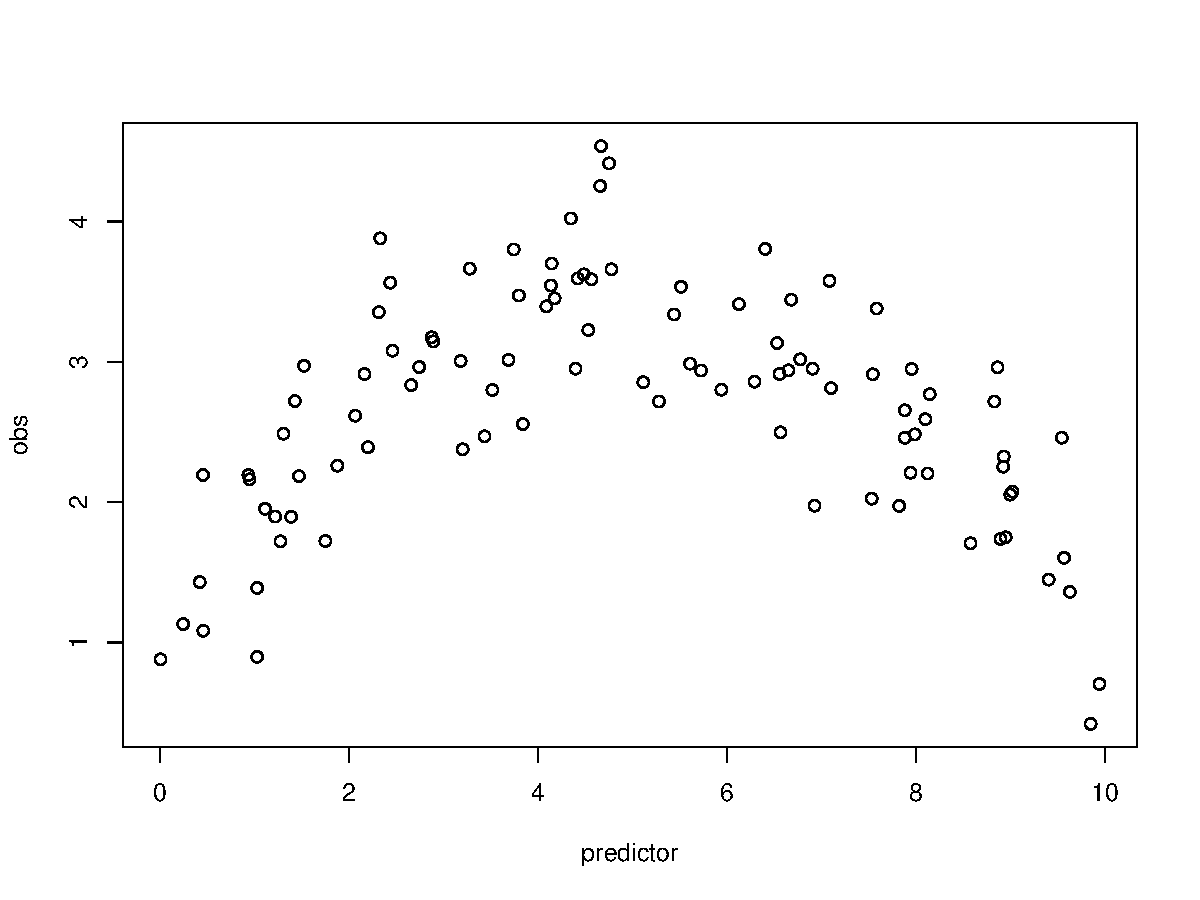
\includegraphics[width=0.8\textwidth,height=0.6\textwidth]{figure/unnamed-chunk-13-1} 

\end{knitrout}
\end{frame}
%%%%%%%%%%

\begin{frame}[fragile]{Linear regression}

\begin{knitrout}
\definecolor{shadecolor}{rgb}{0.843, 0.867, 0.922}\color{fgcolor}\begin{kframe}
\begin{alltt}
\hlstd{fitlm} \hlkwb{<-} \hlkwd{lm}\hlstd{(}\hlkwc{data} \hlstd{= dat.behav,} \hlkwc{formula} \hlstd{= activity} \hlopt{~} \hlstd{weather)}
\hlkwd{summary}\hlstd{(fitlm)}
\end{alltt}
\begin{verbatim}

Call:
lm(formula = activity ~ weather, data = dat.behav)

Residuals:
    Min      1Q  Median      3Q     Max 
-2.3547 -0.6028  0.2346  0.6419  1.6534 

Coefficients:
             Estimate Std. Error t value Pr(>|t|)    
(Intercept)    6.7815     0.4581  14.805 3.94e-16 ***
weathersunny  -1.6204     0.4948  -3.275  0.00248 ** 
---
Signif. codes:  0 '***' 0.001 '**' 0.01 '*' 0.05 '.' 0.1 ' ' 1

Residual standard error: 1.024 on 33 degrees of freedom
Multiple R-squared:  0.2453,	Adjusted R-squared:  0.2224 
F-statistic: 10.73 on 1 and 33 DF,  p-value: 0.002485
\end{verbatim}
\end{kframe}
\end{knitrout}
\end{frame}
%%%%%%%%%%%

\begin{frame}[fragile]{Regression, graphically}
\textbf{Rate of change}
\centering
\begin{knitrout}
\definecolor{shadecolor}{rgb}{0.843, 0.867, 0.922}\color{fgcolor}
\includegraphics[width=0.8\textwidth,height=0.6\textwidth]{figure/unnamed-chunk-15-1} 

\end{knitrout}
\end{frame}
%%%%%%%%%%


\begin{frame}[fragile]{NB: aov() vs. anova()}

\begin{knitrout}
\definecolor{shadecolor}{rgb}{0.843, 0.867, 0.922}\color{fgcolor}\begin{kframe}
\begin{alltt}
\hlkwd{aov}\hlstd{(}\hlkwc{data} \hlstd{= dat.behav,} \hlkwc{formula} \hlstd{= activity} \hlopt{~} \hlstd{weather)}
\hlkwd{anova}\hlstd{(fitlm)}
\end{alltt}
\end{kframe}
\end{knitrout}

\end{frame}
%%%%%%%%%%%

\begin{frame}{All is one\dots}
\pause
  \begin{block}{\dots but \texttt{lm()} rules!}
    \begin{itemize}
      \item t-test, ANOVA, regression and others can be mathematically equivalent
      \item In R, \texttt{lm()} and related functions can do them all\dots
      \item \dots and much more!
    \end{itemize}
  \end{block}
\end{frame}
%%%%%%%%%%%

%%%%%%%%%%%%%%%%%%%%%%%%%%%%%%%%%%%%%%%%%%%%%%%%%%%%%%%%%%%%%%%%%%%
%%%%%%%%%%%%%%%%%%%%%%%%%%%%%%%%%%%%%%%%%%%%%%%%%%%%%%%%%%%%%%%%%%%
\section{Linear models in details}

\begin{frame}[fragile]{A simple linear model}
  \textbf{{\color{purple}{Response}} = {\color{blue}{Intercept}} + {\color{red}{Slope}} $\times$ {\color{orange}{Predictor}} + {\color{gray}{Error}}} \\
  
\begin{knitrout}
\definecolor{shadecolor}{rgb}{0.843, 0.867, 0.922}\color{fgcolor}
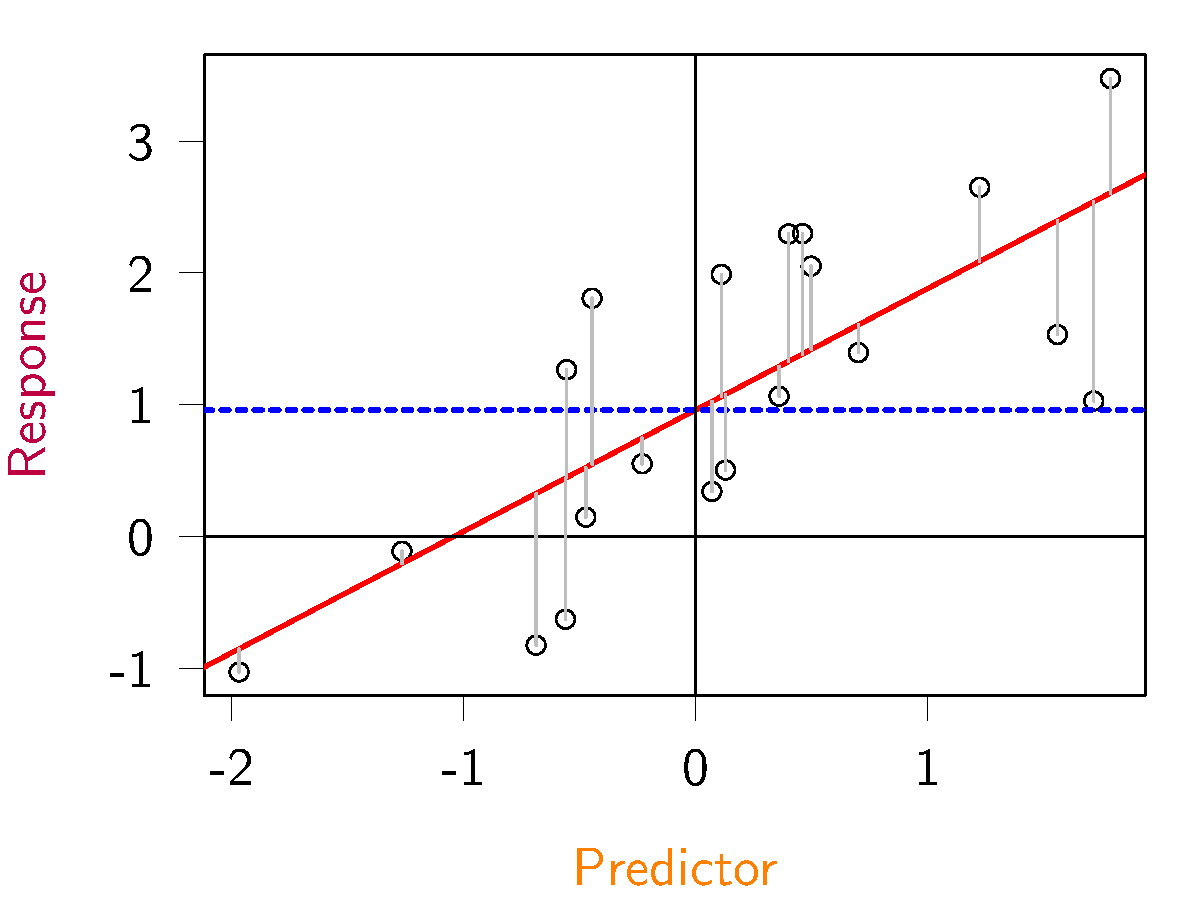
\includegraphics[width=0.8\textwidth,height=0.6\textwidth]{figure/lmprinc-1} 

\end{knitrout}
\end{frame}
%%%%%%%%%%%

\begin{frame}[fragile]{A simple linear model}
  \textbf{{\color{purple}{Response}} = {\color{blue}{Intercept}} + {\color{red}{Slope}} $\times$ {\color{orange}{Predictor}} + {\color{gray}{Error}}} \\
  \vspace{1cm}
\textbf{In R:}
\begin{knitrout}
\definecolor{shadecolor}{rgb}{0.843, 0.867, 0.922}\color{fgcolor}\begin{kframe}
\begin{alltt}
  \hlkwd{lm}\hlstd{(response} \hlopt{~} \hlnum{1} \hlopt{+} \hlstd{predictor1} \hlopt{+} \hlstd{predictor2,} \hlkwc{data}\hlstd{=data)}
    \hlcom{# equivalent to}
  \hlkwd{lm}\hlstd{(response} \hlopt{~} \hlstd{predictor1} \hlopt{+} \hlstd{predictor2,} \hlkwc{data}\hlstd{=data)}
\end{alltt}
\end{kframe}
\end{knitrout}
\begin{itemize}
  \item Intercept can be explicit or implicit
  \item Can remove intercept with \texttt{\dots $\sim $ 0 + \dots}
  \item Error is implicit
  \item Feed the option \texttt{data=} to keep code short, reliable and flexible
  \item Order of predictors do not matter 
\end{itemize}

\end{frame}
%%%%%%%%%%%

\begin{frame}[fragile]{Interpretation}

\begin{knitrout}
\definecolor{shadecolor}{rgb}{0.843, 0.867, 0.922}\color{fgcolor}\begin{kframe}
\begin{alltt}
  \hlstd{Ans} \hlkwb{<-} \hlkwd{read.csv}\hlstd{(}\hlkwc{file} \hlstd{=} \hlstr{"Anscombe.csv"}\hlstd{)}
\end{alltt}
\end{kframe}
\end{knitrout}
  
\begin{knitrout}
\definecolor{shadecolor}{rgb}{0.843, 0.867, 0.922}\color{fgcolor}\begin{kframe}
\begin{alltt}
  \hlstd{lm1} \hlkwb{<-} \hlkwd{lm}\hlstd{(y} \hlopt{~} \hlstd{x ,} \hlkwc{data}\hlstd{=Ans[Ans}\hlopt{$}\hlstd{distri}\hlopt{==}\hlnum{1}\hlstd{,])}
  \hlkwd{summary}\hlstd{(lm1)}
  \hlkwd{plot}\hlstd{(Ans}\hlopt{$}\hlstd{x[Ans}\hlopt{$}\hlstd{distri}\hlopt{==}\hlnum{1}\hlstd{], Ans}\hlopt{$}\hlstd{y[Ans}\hlopt{$}\hlstd{distri}\hlopt{==}\hlnum{1}\hlstd{],}
       \hlkwc{xlim}\hlstd{=}\hlkwd{c}\hlstd{(}\hlnum{0}\hlstd{,}\hlnum{15}\hlstd{),} \hlkwc{ylim}\hlstd{=}\hlkwd{c}\hlstd{(}\hlnum{0}\hlstd{,}\hlnum{12}\hlstd{))}
  \hlkwd{abline}\hlstd{(lm1)}
\end{alltt}
\end{kframe}
\end{knitrout}
\end{frame}
%%%%%%%%%%%

\begin{frame}[fragile]{Interpretation}

 \begin{alertblock}{lm vs. plot}
 \begin{itemize}
   \item Fit a linear model $y \sim x $ for each of the four ``distri"
   \item Plot the relationship  $ y \sim x $ for each of the four ``distri"
   \item Can we trust these models? For what? \textit{\tiny I expect more than ``it's all bullshit"}
  \end{itemize}
 \end{alertblock}

\end{frame}
%%%%%%%%%%%

\begin{frame}{General approach}

\begin{center}
  \begin{tikzpicture}
    \node (sq) at (0,-1) {\color{red}{1. Scientific question}};
    \node (mo) at (0,-2) {2. Model and Statistical question};
    \draw[->, thick] (sq)--(mo);
    \node (dac) at (6,-2) {\color{red}{3. Data collection}};
    \draw[<->, thick] (mo)--(dac);

    \node (est) at (0,-3) {4. Estimation};
        \draw[->, thick] (mo)--(est);
    \node (unc) at (0,-3.5) {4.b Uncertainty and statistical significance};
    
    \node (che) at (0,-5) {\textbf{5. Diagnostic, check assumptions, prediction}};
        \draw[->, thick] (unc)--(che);
    \draw[->, thick] (che.west) to [out=150, in=210] (mo.west);

    \node (int) at (0,-6) {\color{red}{6. Interpret and think about the biology}};
        \draw[->, thick] (che)--(int);

  \draw[rounded corners, color=blue] (-4.5,-1.5) rectangle (4,-5.5);
  \node[anchor=north west] (r) at (-4.5,-1.5) {
\includegraphics[width=0.1\textwidth]{Figures/r}};
  \end{tikzpicture}
  \end{center}
\end{frame}
%%%%%%%%%%%

\begin{frame}{Linear model basic assumptions}
Not necessarily wrong, but typical interpretation assumes:
 \begin{block}{}
     \begin{itemize}[<+->]
      \item Linear combination of parameters (including transformation, polynoms, interactions\dots)\\ \textit{Risk: biologically meaningless}
      \item Predictor not perfectly correlated \\ \textit{Risk: Model won't run, unstable convergence, or huge SE}
       \item {\color{red!20!black}{Little error in predictors}}\\ \textit{Risk: bias estimates (underestimate with Gaussian error)}
       \item {\color{red!50!black}{Gaussian error distribution}}\\ \textit{Risk: Poor predictions}
       \item {\color{red!70!black}{Homoscedasticity (constant error variance)}}\\ \textit{Risk: Over-optimistic uncertainty, unreliable predictions}
       \item {\color{red!99!black}{Independence of error}}\\ \textit{Risk: Bias and over-optimistic uncertainty}
     \end{itemize}
 \end{block}
\end{frame}
%%%%%%%%%%%

\begin{frame}[fragile]{Diagnostic: summary and plot}
\begin{knitrout}
\definecolor{shadecolor}{rgb}{0.843, 0.867, 0.922}\color{fgcolor}\begin{kframe}
\begin{alltt}
 \hlstd{lm1} \hlkwb{<-} \hlkwd{lm}\hlstd{(y} \hlopt{~} \hlstd{x ,} \hlkwc{data}\hlstd{=Ans[Ans}\hlopt{$}\hlstd{distri}\hlopt{==}\hlnum{1}\hlstd{,])}
 \hlstd{lm2} \hlkwb{<-} \hlkwd{lm}\hlstd{(y} \hlopt{~} \hlstd{x ,} \hlkwc{data}\hlstd{=Ans[Ans}\hlopt{$}\hlstd{distri}\hlopt{==}\hlnum{2}\hlstd{,])}
\end{alltt}
\end{kframe}
\end{knitrout}
  
  
\begin{knitrout}
\definecolor{shadecolor}{rgb}{0.843, 0.867, 0.922}\color{fgcolor}\begin{kframe}
\begin{alltt}
 \hlkwd{summary}\hlstd{(lm1)}
 \hlkwd{par}\hlstd{(}\hlkwc{mfrow}\hlstd{=}\hlkwd{c}\hlstd{(}\hlnum{2}\hlstd{,}\hlnum{2}\hlstd{))}
 \hlkwd{plot}\hlstd{(lm1)}
\end{alltt}
\end{kframe}
\end{knitrout}
  
\begin{knitrout}
\definecolor{shadecolor}{rgb}{0.843, 0.867, 0.922}\color{fgcolor}\begin{kframe}
\begin{alltt}
  \hlkwd{summary}\hlstd{(lm2)}
 \hlkwd{plot}\hlstd{(lm2)}
  \hlkwd{par}\hlstd{(}\hlkwc{mfrow}\hlstd{=}\hlkwd{c}\hlstd{(}\hlnum{1}\hlstd{,}\hlnum{1}\hlstd{))}
\end{alltt}
\end{kframe}
\end{knitrout}

\end{frame}

\begin{frame}[fragile]{Diagnostic: prediction}
\begin{knitrout}
\definecolor{shadecolor}{rgb}{0.843, 0.867, 0.922}\color{fgcolor}\begin{kframe}
\begin{alltt}
\hlstd{pred2} \hlkwb{<-} \hlkwd{predict}\hlstd{(lm2,} \hlkwc{se.fit} \hlstd{=} \hlnum{TRUE}\hlstd{,} \hlkwc{interval} \hlstd{=} \hlstr{"confidence"}\hlstd{)}
\hlstd{pred2} \hlkwb{<-} \hlkwd{cbind}\hlstd{(Ans[Ans}\hlopt{$}\hlstd{distri}\hlopt{==}\hlnum{2}\hlstd{,], pred2)}
\end{alltt}
\end{kframe}
\end{knitrout}

\pause
\begin{knitrout}
\definecolor{shadecolor}{rgb}{0.843, 0.867, 0.922}\color{fgcolor}
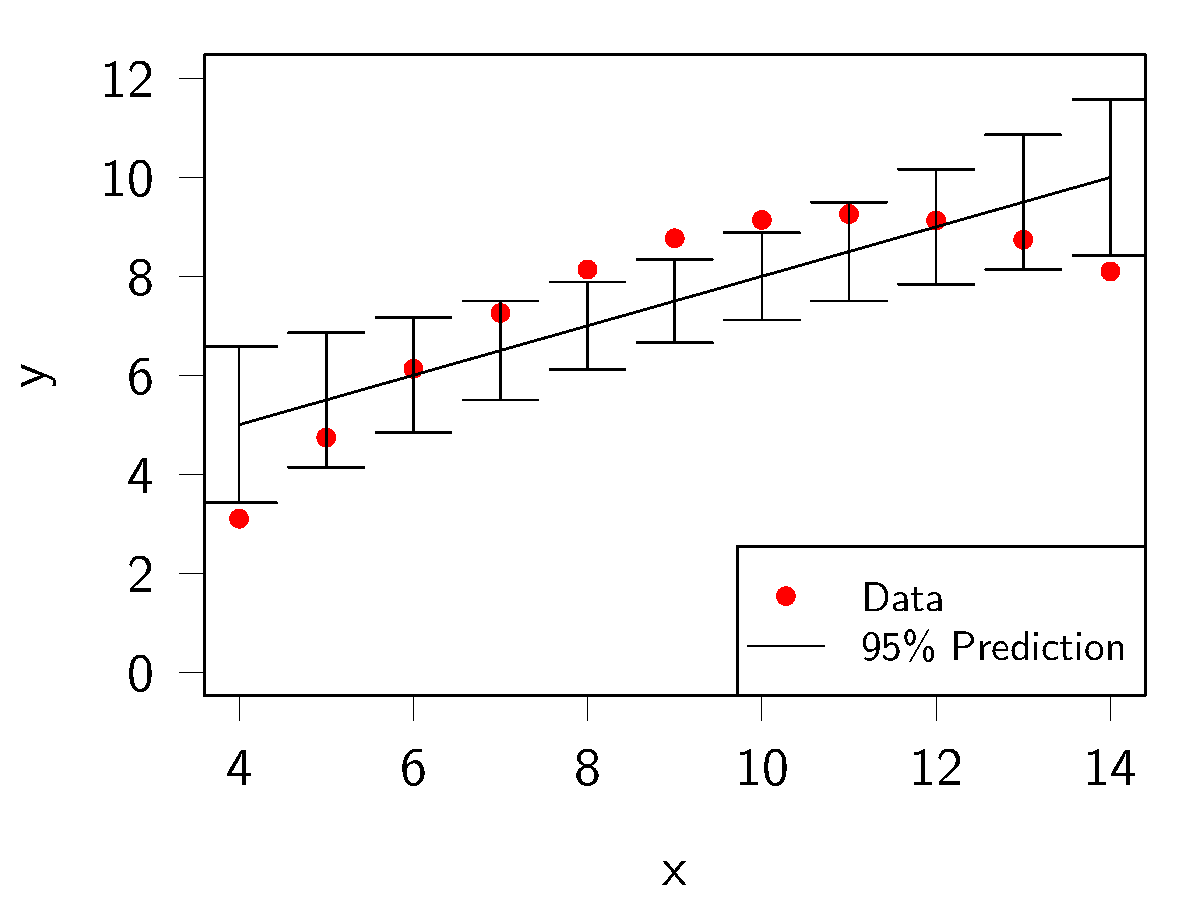
\includegraphics[width=0.8\textwidth,height=0.6\textwidth]{figure/pred2-1} 

\end{knitrout}
\end{frame}
%%%%%%%%%%%

\begin{frame}[fragile]{Practice lm() with parasites}


  
  \begin{alertblock}{What explains variation in parasitic load?}
  You collected ecto-parasites on some furry large mammals at three locations. Parasites break easily when we collect them and are impossible to count, so we decide to measure parasitic load as their mass. \textbf{Why do some mammals have larger parasitic load?} \pause
    \begin{itemize}
      \item Load the \texttt{Para.csv} data (don't forget: str(), summary(), plot()\dots)
      \item Model \verb+Parasite_Mass+ using \texttt{lm()}
      \item Find what variables predict \verb+Parasite_Mass+
      \item How good are your models? Assumptions? Prediction?
      \item What biological interpretation can you imagine?
      \end{itemize}
  \end{alertblock}
  
\end{frame}
%%%%%%%%%%%%%%%%%%%%%%%%%%%%%%%%%%%%%%%%%%%%%%%%%%%%%%%%%%%%%%%%%%%%%%%%%%%%%%%%%
%%%%%%%%%%%%%%%%%%%%%%%%%%%%%%%%%%%%%%%%%%%%%%%%%%%%%%%%%%%%%%%%%%%%%%%%%%%%%%%%%
\section{Bonus fun}
\begin{frame}{Extra exercises}



\begin{alertblock}{General R coding}
  \begin{enumerate}
    \item What is the fastest way to get row averages in a data-frame?
    \item Create a function called colVars, like colMeans but for variance
    \item Create nice plots to visualize iris data (ideally journal-quality)
  \end{enumerate}
\end{alertblock}

\begin{alertblock}{Linear models}
  \begin{enumerate}
    \item Load Cdata.csv, fit models of y predited by x1 and x2, or x2 and x3. Something is weird, what is going on? What to do?
    \item For model that can be fitted with t.test, aov, and lm, is one of the function faster?
    \item Write your own code to obtain a prediction from a lm (that is, a simpler version of the predict function), with confidence interval. (extra toughness: do it using the matrix formulation of the analytical solution to a linear model)
  \end{enumerate}
\end{alertblock}
\end{frame}
%%%%%%%%%%%


\end{document}
